\documentclass[12pt,a4paper]{article}
\title{APG4011F Free Network Practical Report}
\date{21 April 2015}
\author{Tim Marsh}

\usepackage{amsmath}
\usepackage{graphicx}
\usepackage{float}
\usepackage{textcomp}
\usepackage{siunitx}
\usepackage{wrapfig}
\usepackage{caption}
\usepackage{subcaption}

%\usepackage[margin=1in]{geometry}

\graphicspath{ {./} }
\begin{document}
	
	\pagenumbering{gobble}
	\maketitle
	\begin{figure}[H]
		\centering
		
\includegraphics[width=0.7\linewidth]{images/UCTcircular_logo1_CMYK}
		\label{fig:UCTcircular_logo1_CMYK}
	\end{figure}
	\newpage
	\pagenumbering{arabic}
	\tableofcontents
%	\listoffigures
	\newpage
	
	
	\section{Introduction}
	
	This assignment was to Practically do a free network adjustment over 2 epochs and to determine if there had been deformation between the two epochs. this would take way to long if we were to wait for deformation to actually happen so in order to speed up the process the two epochs were a few minutes apart and we moved some of the points manually in a random direction and an unknown distance.
	
	There were 10 points in total with 4 of those being treated as control points and the rest as survey points. Of those remaining 6 points that weren't control, 3 of them were moved.\\
	\begin{minipage}{0.5\linewidth}

	\begin{figure}[H]
		\centering
		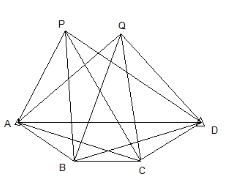
\includegraphics[width=0.6\linewidth]{images/unnamed}
		\label{fig:figure}
	\end{figure}

	\end{minipage}
	\begin{minipage}{0.5\linewidth}
		
	The diagram along side shows a simplified version of the network used in this assignment. The points A,B,C,D are control points and the points P and Q (There are more points in this assignment not only P and Q) are survey points.
		
	\end{minipage}
	
	\section{Background to the Problem}
	
	We did the observations of this assignment using forced centering, this is where we have all our control points set up with tripods with tribrach's on each tripod. that way no pegs need to be placed and moving setups is very fast. 
	
	In a parametric adjustment of a survey network points must be held fixed so that the network can be adjusted to fit those points. If there are no points held fixed it will become impossible to solve the least squares adjustment because there will be a rank defect in the $A^TPA$ Matrix. This means that $A^TPA$ is singular and therefore not invertible.
	
	A free network does exactly that. Keeps no points fixed and winds up with a singular $A^TPA$ Matrix. it however solves this by introducing the $G$ Matrix.
	
	The $G$ matrix contains the eigenvectors of $A^TPA$ for all eigenvalues $\lambda = 0$.
	
	Other than the introduction of the $G$ Matrix the two adjustments are very similar in format.\\
	\\
	Once a free network is calculated from observations from both epochs it is time to try determine if a deformation has occurred. there are two base methods to do this
	\begin{description}
		\item [The X-method] or coordinate method. The x-method relies on the comparison of point coordinates for the various epochs. The basis of the comparison is the assumption that deformations in th point field will result in a shift of the point x-y coordinates
		
		\item [The l-method] or invariant functions method. the l-method compares those quantities of the various epoch networks which are invariant to change of the reference system. in a 2D network the invariant quantities are distances and angles (not directions).
		
		it is referred to as the l-method as the compared quantities are observable in the least squares model and and the letter 'l' is usually associated with observations.
	\end{description}

	\section{Method}
	
		\subsection{Free Network Adjustment}
	
			Free Network Adjustment starts by calculating $N$ where $N$ is:
			\begin{equation}
			\notag
			N = A^TP_{\ell\ell}A
			\end{equation}
			A has the same form as in the parametric adjustment, the $P_{\ell\ell}$ Matrix is the weights of the observations as opposed to $P_{bb}$ which is the vector of pseudo-observations. $P_{bb}$ is usually set to an identity so that it falls away from the equations.
			
			Once $N$ is created. we then need to calculate $G$. The $G$ matrix contains the eigenvectors of $N$ for all eigenvalues $\lambda = 0$.
			\\
			Then $\bar{N}$ is calculated using $N$ and $G$:
			\begin{equation}
			\notag
			\bar{N} = A^TPA + GG^T
			\end{equation}
			\\
			inverting that to get $\bar{Q}$:
			\begin{equation}
			\notag
			\bar{Q} = \bar{N}^{-1} = (A^TPA + GG^T)^{-1}
			\end{equation}
			\\
			And then finally $X$ is found:
			\begin{equation}
			\notag
			X = \bar{Q} A^TP\ell	
			\end{equation}
			\\
			The in order for us to compare Parametric and Free Network we need to hold two points fixed, this is done with an S-Transformation.
			
			An S-Transform makes it possible to transform the x-Vector and Q-Matrix of a free network adjustment into any minimum constrained datum and visa versa.
			
			To get $X_2$, the constrained $X$, we need to transform $X_1$ using G and a selective identity matrix.
			\begin{equation}
			\notag
			X_2 = X_1 - G(G^TI_sG)^{-1} G^T I_s X_1
			\end{equation}
			The selective identity matrix is mostly zeros and has 1's along the diagonal in line with the elements in the $X_1$ Matrix that we want to keep fixed.
			
			After the network has been calculated for both epochs a deformation analysis is then preformed on the point field.
	
		\subsection{The Hanover Approach}
			The Hanover approach utilizes the X-method and attempts to answer 3 questions:
			\begin{enumerate}
				\item Have the points shifted?
				\item Which points have shifted?
				\item What from does the deformation have? (if there is one)
			\end{enumerate}
		~\\
		The steps involved in the Hanover approach are as follows:
		
			\subsubsection{The Free Network Adjustment}
			
				As explained above
				
			\subsubsection{The Global Test}
			
				The global test determines if deformations have taken place.
				
			\subsubsection{Test for Deformations}
				A fisher distribution is used to test the variance of the two epochs against each other. to see if a deformation has occurred.
				
			\subsubsection{Identification of Stable points}	
				
				Then once it has been determined that a deformation has occurred you need to identify the stable points and creating a set of stable points as well as a set of unstable points.
				
			\subsubsection{Determination of the deformation vector - Twin point adjustment}
				The final step of the analysis is to quantify the deformation. A simple method of achieving this is the twin point method.
				
				The concept is to adjust both epochs in on network adjustment and to introduce points, which have been identified as possibly unstable as two separate points (twin points). This means that double observations exist between the stable points strengthening their determination, while each of the suspect points is determined as two separate 'twin points'.
			
	
	\section{Conclusion}
		The aim of this report was to conduct and understand deformation analysis from the ground up. and the process was followed as outlined above. there are other methods but this was the method that fitted best.
	
	
	
\end{document}